% !TeX root = ..\essay.tex

% Notes from slides

% Erfolg der Methode
% 	Nutzung der Methode in der Literatur
% 	Ergebnisse auf anderen Corpora/Daten
% Literaturrecherche
% 	Erweiterungen der Methode
% 	Kritik der Methode
% Ver-/Anwendung der Methode
% theoretischer Bezug
% Praktischer Bezug
% Verwendbarkeit
% Beschreibung der Methodik
% Bewertung der Methode
% Verwendung von (Fach-)Begriffen richtig und konsistent
% Mit eigenen Worten
% Wissenschaftliches Arbeiten
% Korrekte Zitierweise
% Weiterfuehrende Ideen und Gedanken

% What is the prob­lem that the au­thors tried to solve in this paper?
% How does this prob­lem re­late to the topic of the sem­i­nar and to other talks in the sem­i­nar?
% How can I ex­plain the au­thors' so­lu­tion in the best way?
% How did the au­thors demon­strate that the so­lu­tion works?


\subsection{Step 2 - Creating Hierarchies}

\subsection{Introduction}

In the second step of our pipeline we created tree hierarchies out of the sentences that were selected in the first step. The results of the content selection created a list of sentences for each topic. Our system took those sentences and created a tree with each branching tree indicating a new sub topic. Each node of a tree contained one or more sentences. At the top is a root level with multiple trees that differ in the topics of their sentences. 

The tree hierarchies are build for the third step to better distinguish between topics of sentences. Each resulting tree should contain sentences that are similar in meaning and topic. At the top of each tree should be the most general sentence and at the bottom the most specific sentence.


\subsection{Method}

Our method can be descriped in three steps. First we defined an recursive function to insert an sentence into the resulting tree. Then we defined two functions to determinate where to go in the tree. These functions also implement how similarity and specific/general sentences are calculated.

\textbf{Insert}\\

% TODO: insert images
\begin{figure}[H]
	\centering
	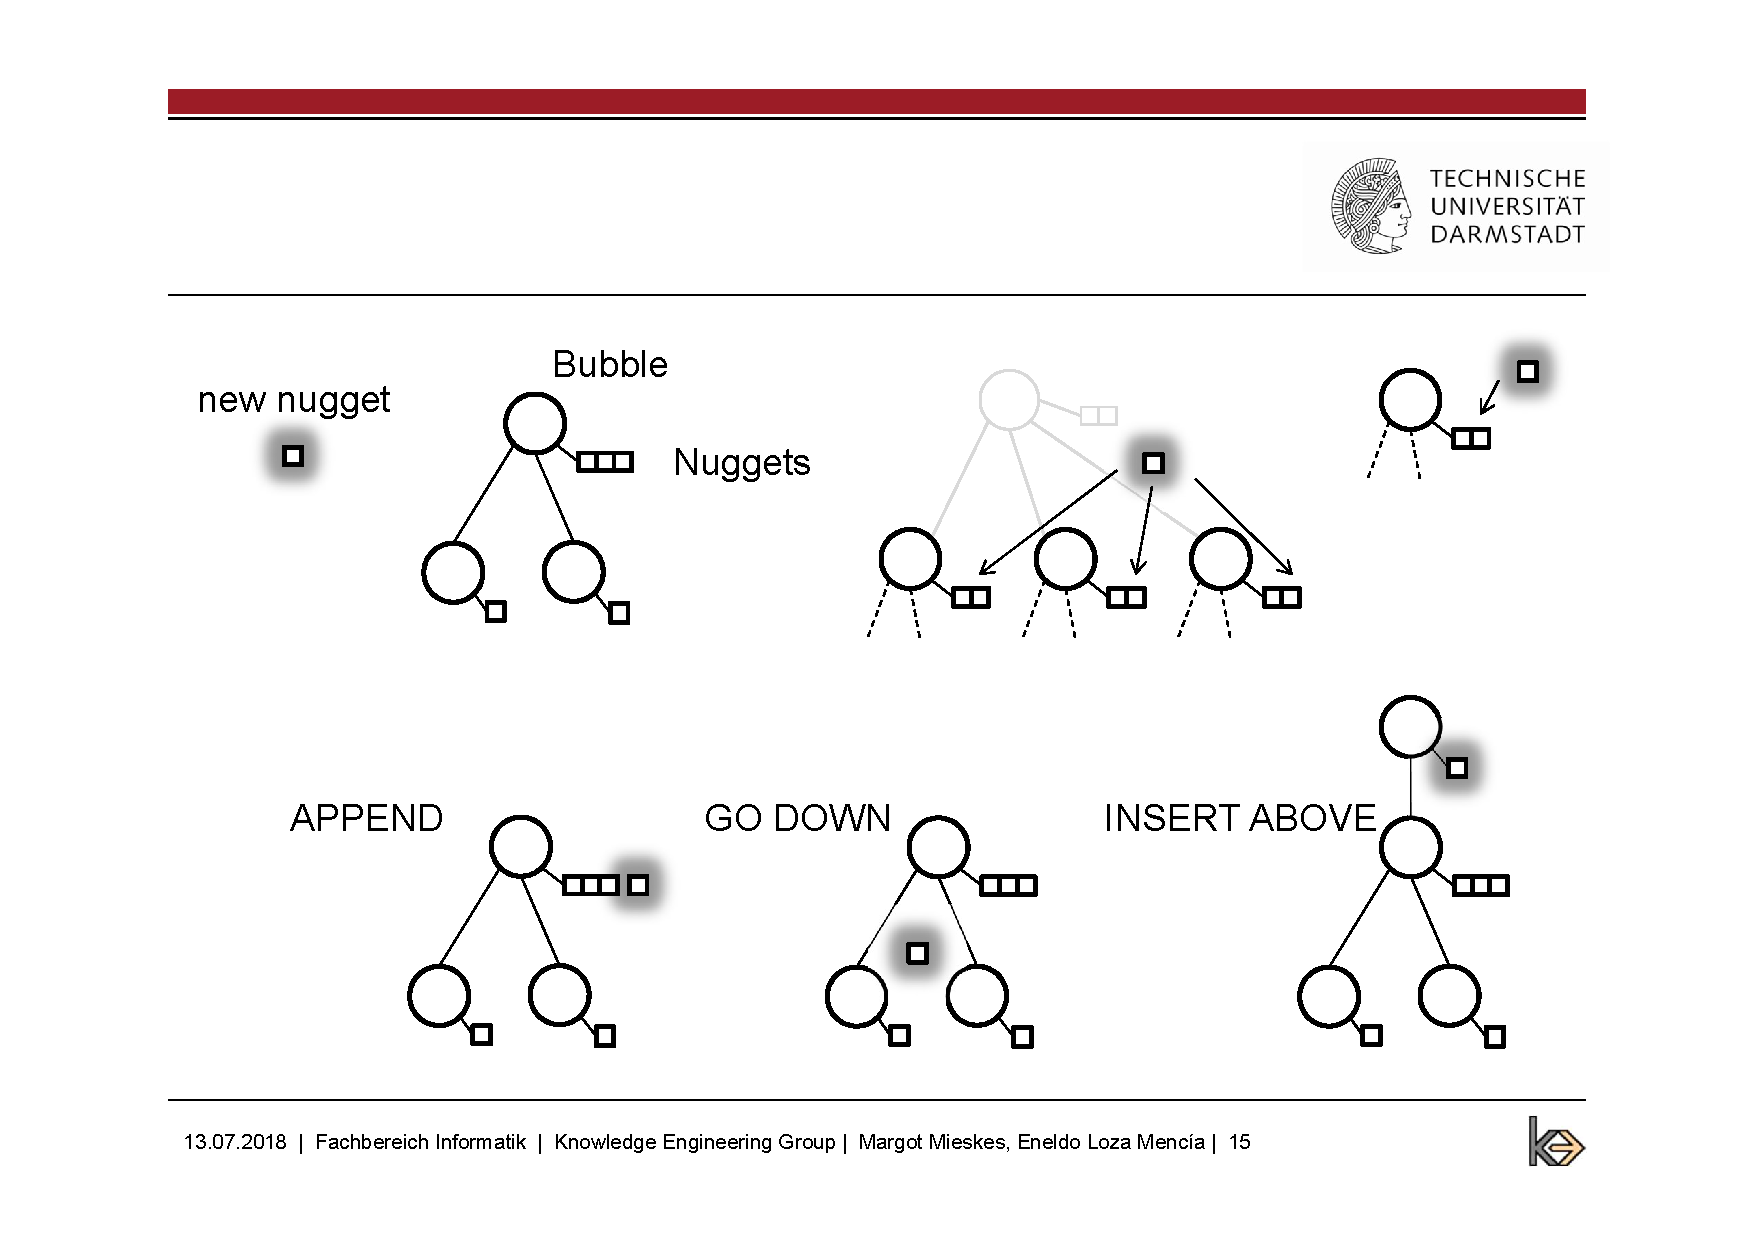
\includegraphics[trim=3cm 10cm 15cm 5.8cm, clip=true, width= \textwidth]{img/step2_func.pdf}
	\caption{Bubble and Nugget}
	\label{fig:jsd}
\end{figure}

\begin{figure}[H]
	\centering
	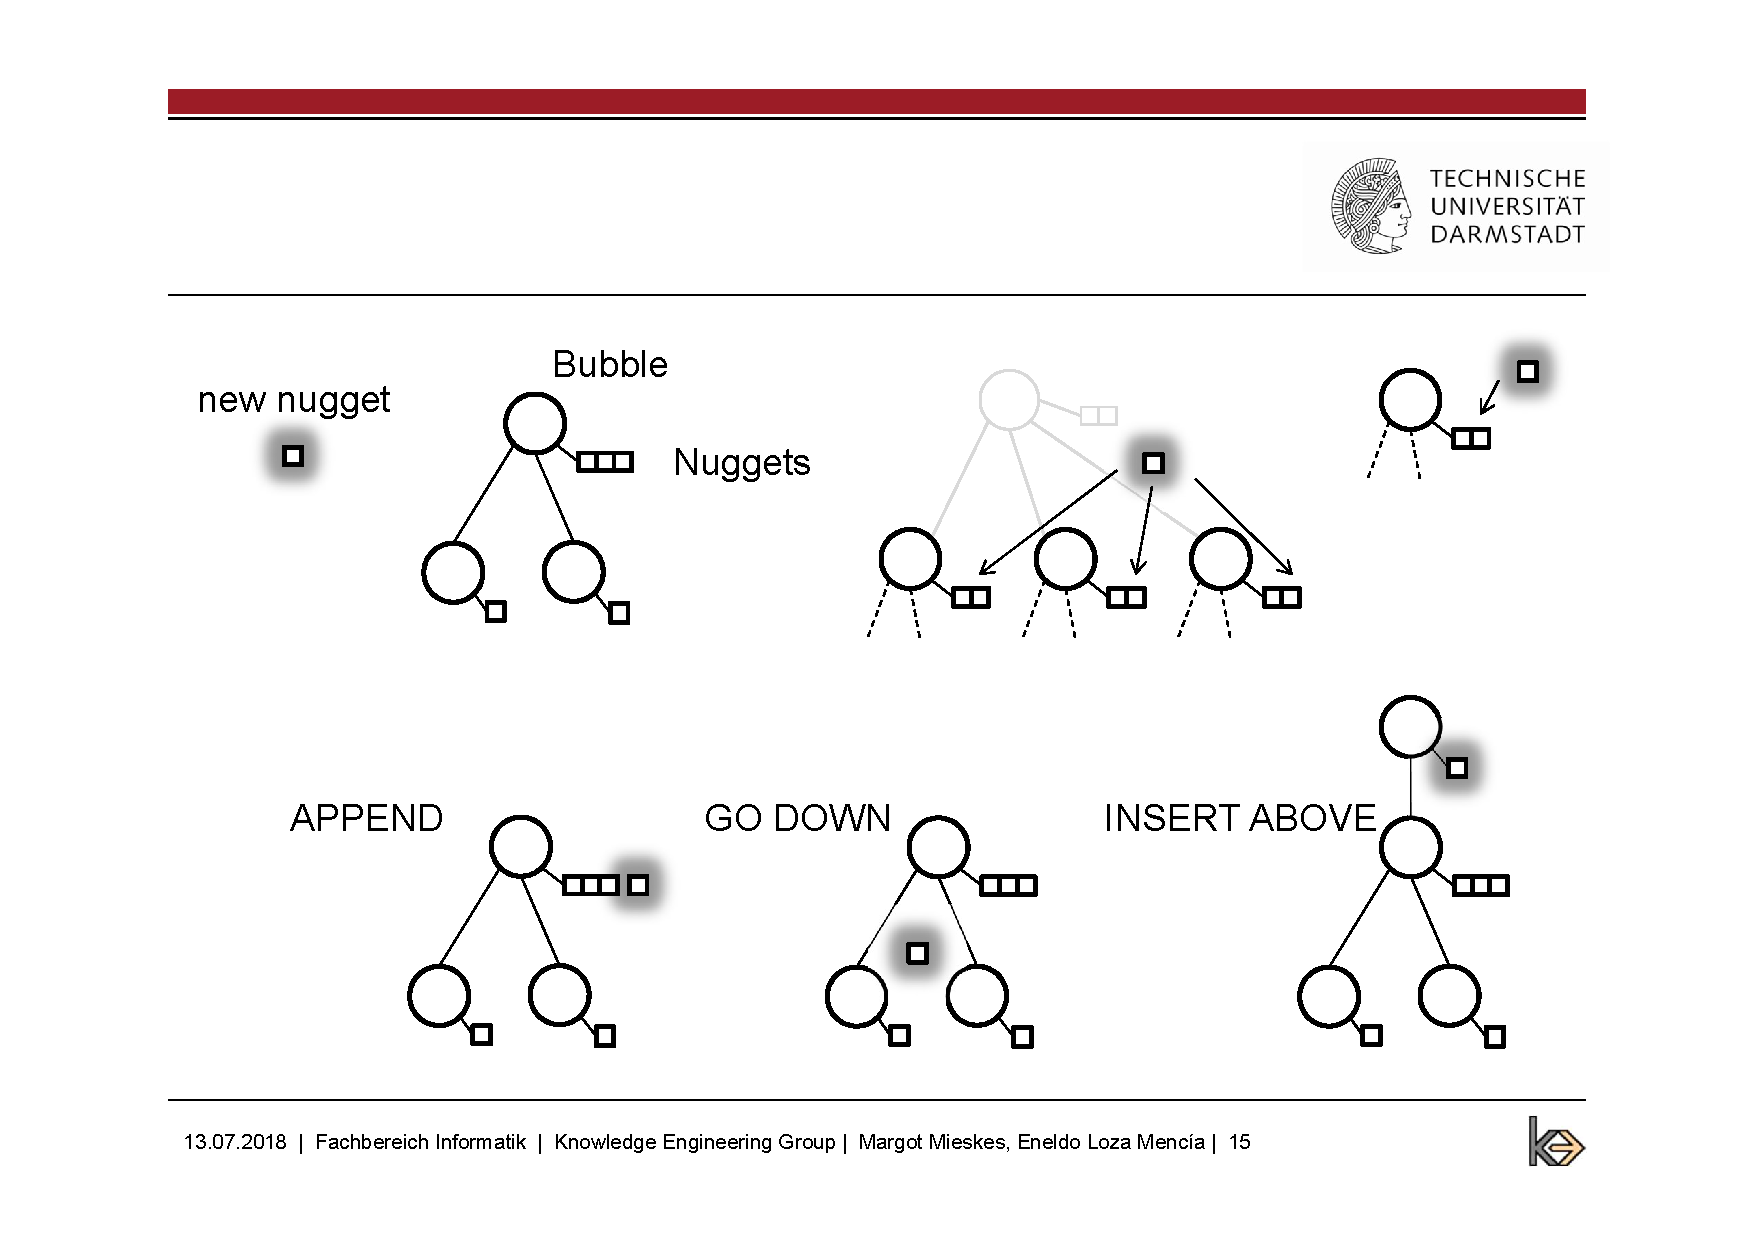
\includegraphics[trim=14cm 10cm 2.5cm 5.5cm, clip=true, width= \textwidth]{img/step2_func.pdf}
	\caption{Insert}
	\label{fig:jsd}
\end{figure}

\begin{figure}[H]
	\centering
	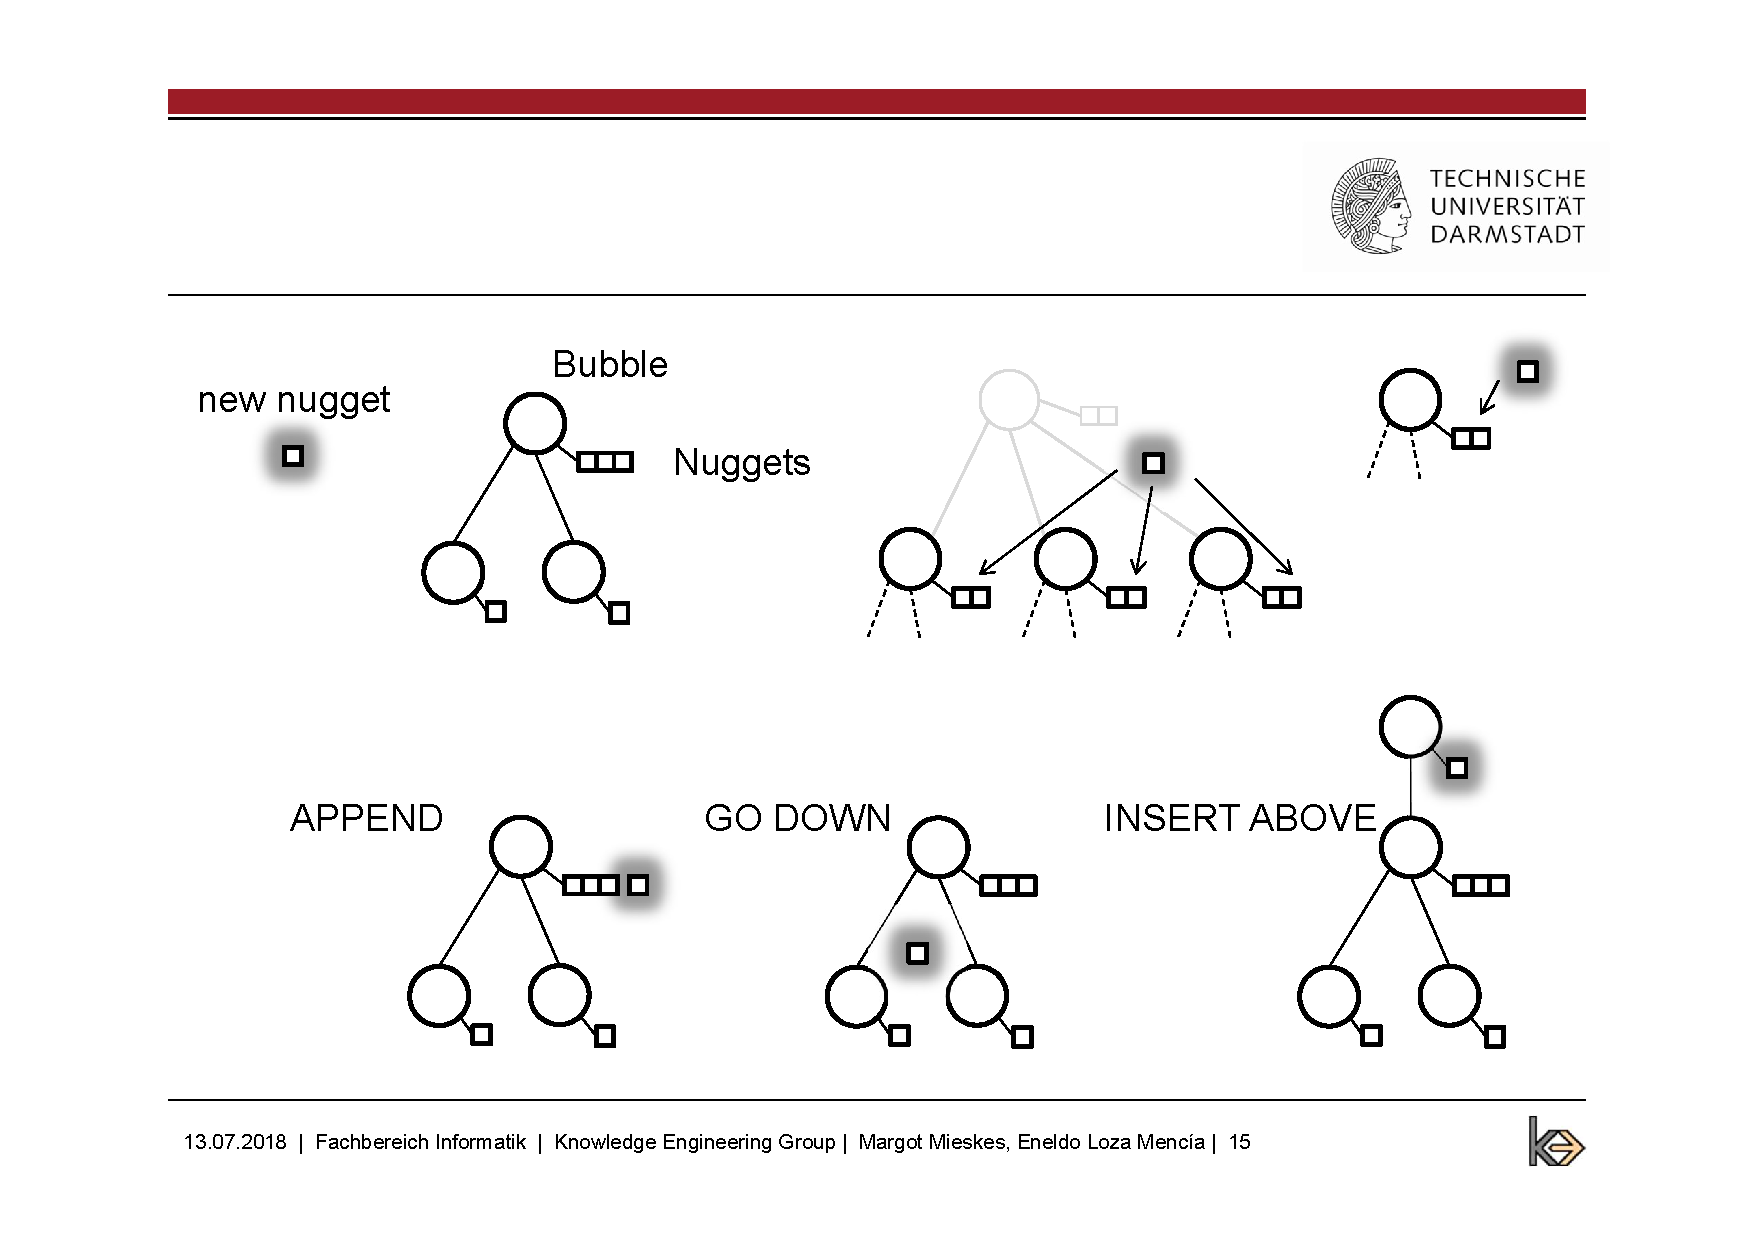
\includegraphics[trim=3cm 3cm 3cm 11cm, clip=true, width= \textwidth]{img/step2_func.pdf}
	\caption{Three Steps}
	\label{fig:jsd}
\end{figure}

The insert function takes a nugget and inserts it into the given tree. It runs resursivly over the tree and calls the Which and Compare functions to determine where to go. Each step it first calls the Compare function which takes the current list of nuggets and the nugget which should be inserted. It returns the position where to insert the given nugget. There are three decicions to consider.

\begin{description}
\item [Append] It appends the given nugget to the current list of nuggets.
\item [Go Down] We call Which to determine in which bubble to go resursivly. The Which function returns the best Bubble to insert. The function then calls itself recursivly in this Bubble.
\item [Insert Above] A new Bubble is created and inserted above the current Bubble and the pointers between the Bubbles are pointed to their new positions.
\end{description}

\textbf{Which}\\

The Which function takes a list of Bubbles and the current Nugget to insert and returns the best position to insert the Nugget. This function tries to find the similarity of each Bubble to the current Nugget. Each Bubble can contain 1 to n Nuggets at the top level and multiple other in their silbings. We only take the 1 to n Nuggets in the top level and compare each word of each Nugget with NLTK path similarity.

% TODO: describe path similarity
% TODO: link nltk webpage
% Return a score denoting how similar two word senses are, based on the shortest path that connects the senses in the is-a (hypernym/hypnoym) taxonomy. The score is in the range 0 to 1. By default, there is now a fake root node added to verbs so for cases where previously a path could not be found---and None was returned---it should return a value. The old behavior can be achieved by setting simulate_root to be False. A score of 1 represents identity i.e. comparing a sense with itself will return 1.

\textbf{Compare}\\

The compare function takes the current list of Nuggets and the Nugget which should be inserted and returns where to insert it (See List of decisions in Insert function). We calculate the TF-IDF scores for the current nugget and the list of nuggets against the whole document. We do this because we want to find which Nugget is more important, aka more general or specific.

% TODO: link original tf idf paper
%In information retrieval, tf–idf or TFIDF, short for term frequency–inverse document frequency, is a numerical statistic that is intended to reflect how important a word is to a document in a collection or corpus.[1] It is often used as a weighting factor in searches of information retrieval, text mining, and user modeling. The tf-idf value increases proportionally to the number of times a word appears in the document and is offset by the frequency of the word in the corpus, which helps to adjust for the fact that some words appear more frequently in general. Tf-idf is one of the most popular term-weighting schemes today; 83% of text-based recommender systems in digital libraries use tf-idf. Variations of the tf–idf weighting scheme are often used by search engines as a central tool in scoring and ranking a document's relevance given a user query. tf–idf can be successfully used for stop-words filtering in various subject fields, including text summarization and classification.

\subsection{Experimental Setup}

We used Python and NLTK.

\subsection{Experimental Results}

We tried Annotation Tool from AIPHES
11 percent similarity average against Gold standard (same as Random Trees)
but
1300 Nuggets in gold standard versus 30 Nuggets we used
less Nuggets showed more similarity
our algorithm is slow (>30 min) with 300+ Nuggets
Find „right“ balance instead
1-5 Nuggets in each Bubble
5+ Bubbles in root node

Show evaluation of AIPHES:
	number of root trees
	Average Depth
	Gold standart vs Random Tree vs our solution

sometimes resulting tree's were strange
therefore remove insert UP from insert, just go down
trust in the pre-sort sentences
pre-sort sentences ourself? step one is already doing that

\subsection{Discussion}

hard to find other papers on this specific topic on building hierarchies
hard to do evaluation of performance on system

Is there a best (gold standard) hierarchy?
Problem: How to define similarity of hierarchies?

future stuff
which and compare function can be improved which improves overall system
do some kind of clustering to insert into 4-5 trees and then use our solution for subtrees
use word vectors or sentence vectors for comparing function

hard to define similar when we want general / specific

\subsection{Conclusions}

3 functions which our algoithm was made of
system results were okay?
hard to messure


%\subsection{Bibliography}
% added at the end